\documentclass{article}
\usepackage[utf8]{inputenc}
\usepackage{graphicx}
\usepackage{amsmath}
\usepackage{amssymb}
\usepackage[utf8]{inputenc}
\usepackage[english]{babel}
\usepackage{amsthm}
\usepackage{makecell,tabularx}
\usepackage{hyperref}
\usepackage{subcaption}

\newtheorem{theorem}{Theorem}[section]
\newtheorem{corollary}{Corollary}[theorem]
\newtheorem{lemma}[theorem]{Lemma}
\theoremstyle{definition}
\newtheorem{definition}{Definition}[section]

\hypersetup{colorlinks,urlcolor=blue}
%% or
% \hypersetup{colorlinks=false,pdfborder=000}

% hack into hyperref
\makeatletter
\DeclareUrlCommand\ULurl@@{%
  \def\UrlFont{\ttfamily\color{blue}}%
  \def\UrlLeft{\uline\bgroup}%
  \def\UrlRight{\egroup}}
\def\ULurl@#1{\hyper@linkurl{\ULurl@@{#1}}{#1}}
\DeclareRobustCommand*\ULurl{\hyper@normalise\ULurl@}
\makeatother

\graphicspath{ {images/} }

\title{Coursera Notes}
\author{Siavash Aslanbeigi}
\date{April 2018}

\begin{document}

\maketitle
\tableofcontents

% INTRODUCTION =========================================
\section{Introduction}
Machine learning is a collection of techniques which allow computers to complete tasks by learning from data. It grew out of work in Artificial Intelligence (AI). Traditionally, we program computers to do what we want by giving them precise instructions. There are problems for which this technique doesn't work very well. 

Consider the problem of recognizing hand-written digits: given an image of a hand-written digit, the computer is supposed to map it to the corresponding digit, i.e. pick correctly from $0,1,\dots,9$. Figure \ref{intro-fig:mnist-examples} shows examples of hand-written digits. It is quite easy for a human to recognize these digits correctly, even though none of them have the exact same shape. Programming a computer to do the same turns out to be difficult. The reason is that it's impossible to explicitly tell the computer about all possible shapes; there are just too many of them. Machine learning approaches this problem differently: we present the algorithm with images like those shown in Figure \ref{intro-fig:mnist-examples} (input), as well as the correct digits they represent (output), and let the algorithm figure out for itself what the correct way of recognizing hand-written digits is. Once the algorithm is trained on the data, we can use it to recognize digits not in the dataset, i.e. to make predictions. This technique has proven more reliable than any other approach. It also seems more inline with how humans learn from experience.

\begin{figure}[ht]
\centering
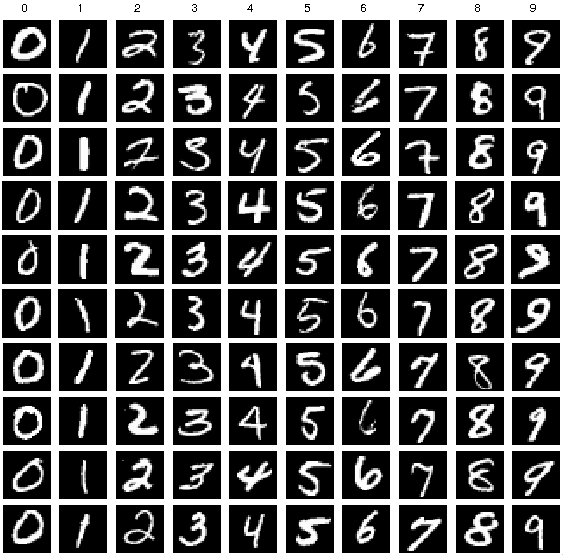
\includegraphics[scale=0.4]{images/intro/mnist-ex.png}
\caption{Examples of handwritten digits from the MNIST dataset.}
\label{intro-fig:mnist-examples}
\end{figure}
Other modern applications of machine learning include:
\begin{itemize}
    \item Spam filters: it is impossible to explicitly list all possible spam emails one might receive.
    \item Database mining: growth of automation/web has resulted in much larger data sets which need to be understood. Examples include web click data, medical records, etc.
    \item Natural Language Processing (NLP), whose aim is to make computers understand text.
    \item Self-customizing programs, such as Netflix product recommendations.
    \item Understanding the human brain. How is it that we humans learn?
\end{itemize}
Here are two formal definitions of machine learning:
\begin{itemize}
    \item Arthur Samuel (1959): Field of study that gives computers the ability to learn without being explicitly programmed. Samuel built a Checkers playing program where the computer would learn from playing tens of thousands of games against itself. This was the world's first self-learning program.
    \item Tom Mitchell (1998): A computer program is said to learn from experience E with respect to some task T and some performance measure P, if its performance on T, as measured by P, improves with experience E.
\end{itemize}
There are two main types of machine learning algorithms: supervised-learning and unsupervised learning.

% Supervised learning ----------------------------------
\subsection{Supervised learning}
Supervised learning is the most common type of machine learning problem. The name \textbf{supervised} comes from the fact that the training samples (i.e. data set) contain the ``right answers". In other words, for a set of inputs, we know what the output should be. Suppose we have the following data for prices of houses:

\begin{figure}[ht]
\centering
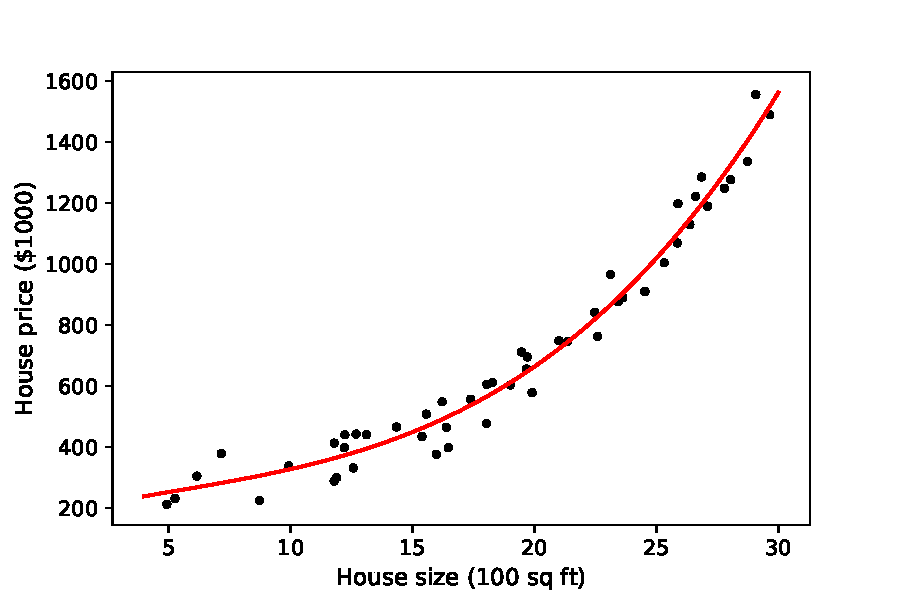
\includegraphics[scale=0.7]{images/lin_reg/poly-data.pdf}
\caption{Predicting house prices.}
\label{into-house-prices}
\end{figure}

What is the price of a house which is $800 \text{ft}^2$? Although none of the houses in our data set have that size, we could make a prediction by fitting a curve through the data points, as shows in Figure \ref{into-house-prices}.

Supervised learning algorithms fall in two broad categories:
\begin{itemize}
    \item \textbf{Regression}: output values are continuous, for instance, predicting house prices, stock prices, etc.
    \item \textbf{Classification}: output values are discrete, for instance whether or not a tumor is malignant or benign.
\end{itemize}

Suppose we have a data set about breast tumors: we are given the size of each tumor, age of the patient, and whether or not it's malignant.

\begin{figure}[ht]
\centering
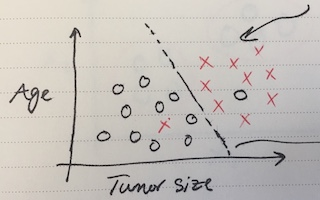
\includegraphics[scale=0.8]{images/intro/tumor.jpg}
\caption{Predicting whether new tumor is malignant or benign. Circles denote benign tumors, and Xs malignant ones.}
\label{intro-tumor}
\end{figure}

Given a new tumor, we'd like to be able to predict whether or not it's malignant or benign. This is an example of a classification problem, since the output values are discrete (we can assign $0$ to benign tumors, and $1$ to malignant ones.) The learning algorithm may decide that the line drawn in Figure \ref{intro-tumor} separates benign and malignant tumors.

% Unsupervised learning --------------------------------
\subsection{Unsupervised learning}
In supervised learning, the training samples tell us the correct outputs for a set of inputs. We then seeks to predict the output for new examples. Unsupervised learning is different in that we not given the right answers. It's more like, here's a data set, find some structure in it. For instance, a learning algorithm may tell us that in Figure \ref{intro-clustering} most of the data is concentrated in two different regions,those which are circled. This is an example of a clustering algorithm.

\begin{figure}[ht]
\centering
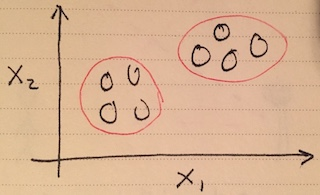
\includegraphics[scale=0.8]{images/intro/clustering.jpg}
\caption{Clustering algorithm.}
\label{intro-clustering}
\end{figure}

A real-life application of clustering is Google News, which looks at thousands of news and groups similar ones together. For instance, it would recognize that these articles from different sources are about the same topic and clusters them together:

\begin{itemize}
    \item The Source: BP kills Macondo, but its legacy lives on.
    \item CNN: Well is dead, but much Gulf Coast work remains.
    \item Guardian: BP oil spill costs nearly $\$10$bn dollars.
\end{itemize}

How remarkable is this? Here's another example of an unsupervised learning algorithm: the cocktail party problem, demonstrated in Figure \ref{intro-cocktail}.

\begin{figure}[ht]
\centering
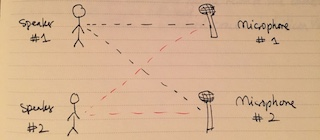
\includegraphics[scale=0.8]{images/intro/cocktail.jpg}
\caption{Cocktail party problem.}
\label{intro-cocktail}
\end{figure}

Two people are talking at the same time. In microphone 1, the sound of speaker 1 is recorded more loudly than speaker 2, simply because speaker 1 is closer to microphone 1, and vice versa for microphone 2. If the volume offsets are pronounced enough, a human would easily recognize by listening to the recording of microphones 1 and 2 that there are two speakers, and even what each of them is saying. The amazing thing is that there are unsupervised learning algorithms that are capable of doing the same. Based on the volume offsets, they recognize the structures of the two speakers sounds and are able to separate them out.


% Linear regression with one variable ==================
\section{Linear regression with one variable}
Consider a \textit{training set} (data set which we'll use to fit parameters of our model, or \textit{train} our model) for house prices in Portland, OR:

\begin{center}
\begin{tabular}{ |c|c| } 
 \hline
 Size ($\text{ft}^2$) (x) & Price ($\$1000$) (y) \\
 \hline
 2104 & 460 \\
 1416 & 232 \\
 1534 & 315 \\
 852 & 178 \\
 \vdots & \vdots \\
 \hline
\end{tabular}
\end{center}

Our job is to learn from this data how to predict prices of houses as a function of their size. This is a supervised learning problem, because our training set contains the right answers: for every input (house size), we know the right output (house price). Moreover, this is a regression problem, because the output variable (house price) is continuous. Figure \ref{linreg-bigpic} shows the picture of how we will tackle this problem: given the training set, our learning algorithm will spits out a function $h$, called the \textit{hypothesis} function, which can estimate the price of a house given its size.

\begin{figure}[ht]
\centering
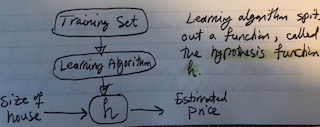
\includegraphics[scale=0.8]{images/lin_reg/big-picture.jpg}
\caption{Big picture.}
\label{linreg-bigpic}
\end{figure}

% Model representation ---------------------------------
\subsection{Model representation}
How do we represent $h$? We start with the simplest function possible and consider more complex models later:
\begin{equation}
    h_{\theta}(x) = \theta_0 + \theta_1 x.
    \label{linreg-eq:univar-hypothesis}
\end{equation}
This function assumes a linear relationship between the size of a house $x$ and its price $h_{\theta}(x)$. We will come up with a learning algorithm that uses the training set to estimate the coefficients $\theta_0$ and $\theta_1$. With that at our disposal, we can predict the price of a house given its size. This learning algorithm is sometimes referred to as \textit{univariate linear regression}, because $h_{\theta}(x)$ is a linear function of a single variable (size of house).

% Cost function ----------------------------------------
\subsection{Cost function}
What values of $\theta_0$ and $\theta_1$ provide the best fit to our data set? Let's start by establishing notation:
\begin{itemize}
    \item $m$: number of training examples.
    \item $x$: input variable/feature (size of house).
    \item $y$: output/target variable (price of house).
    \item $(x^{(i)}, y^{(i)})$: $i$th training example (size and price of $i$th house).
\end{itemize}

For a given house size $x^{(i)}$ in our training set, we know the correct house price $y^{(i)}$. It then makes sense to pick $\theta_0$ and $\theta_1$ so that $h_{\theta}(x^{(i)})$ is as close to $y^{(i)}$ as possible. Realistically, we cannot always pick $\theta_0$ and $\theta_1$ so that $h_{\theta}(x^{(i)})=y^{(i)}$ for all examples, since we only have two parameters to tune, but many more examples to fit, i.e. $m \gg 2$. As a result, we need to strike a balance across all examples, so that the collective prediction error $|h_{\theta}(x) - y|$ on the training set is minimized. To that end, consider the following function, called the \textit{cost function}:

\begin{align}
    J(\theta_0, \theta_1) &= \frac{1}{2m}\sum_{i=1}^{m}(h_{\theta}(x^{(i)}) - y^{(i)})^2
    \label{linreg-eq:costfunc}\\
    &= \frac{1}{2m}\sum_{i=1}^{m}(\theta_0 + \theta_1 x^{(i)} - y^{(i)})^2.
    \label{linreg-eq:univar-costfunc}
\end{align}
Given $\theta_0$ and $\theta_1$, it computes the sum of (squared) prediction errors across all training examples. (It also normalizes the sum by $2m$, but that's only for mathematical convenience.) The lower the value of $J$, the closer the model's prediction to the observed house prices in the training set. So it makes sense to pick $\theta_0$ and $\theta_1$ so that $J$ is minimized. Figure \ref{linreg-fig:costfunc} shows the correspondence between minimizing $J$ and getting a better fit to to the training set. 

\begin{figure}[ht]
\centering
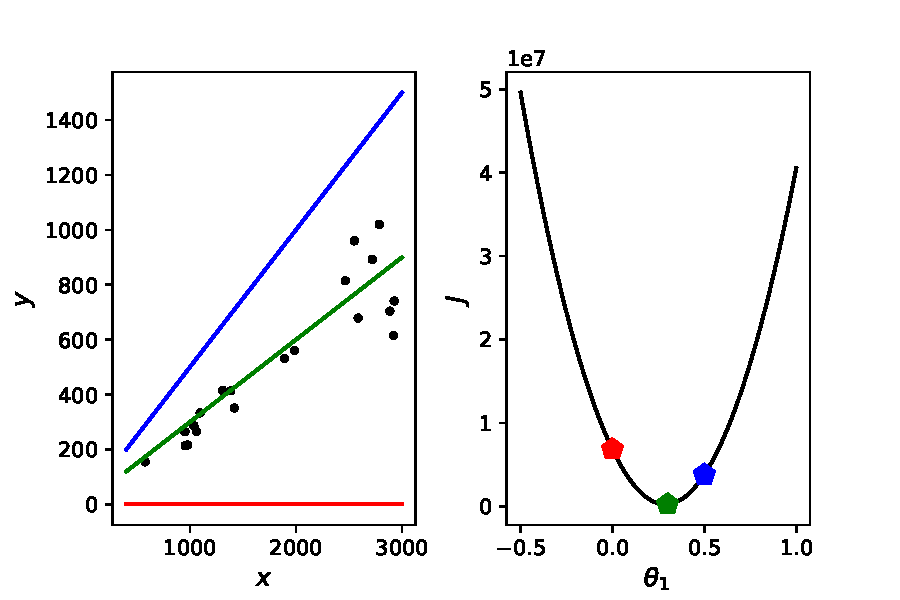
\includegraphics[scale=0.7]{images/lin_reg/costfunc.pdf}
\caption{Correspondence between minimizing the cost function and getting a better fit to data. The following model is used to fit the data: $h_{\theta}(x) = \theta_1 x$. Black dots on the left show the training set. The right figure shows the cost function $J(\theta_1)$. Every dot on the right figure corresponds to a line of the same color on the left figure. We see that the closer $\theta_1$ is to $J$'s minimum, the better the fit to data is. Code used to generate this plot can be found \href{https://github.com/siavashaslanbeigi/ml_notes/blob/master/src/lin_reg/costfunction.ipynb}{here}.}
\label{linreg-fig:costfunc}
\end{figure}

Why cost function \eqref{linreg-eq:univar-costfunc} and not some other one? There are plenty of other cost functions whose minimization would also lead to a good fit of data. For linear regression, though, \eqref{linreg-eq:univar-costfunc} does have some desirable mathematical properties. First of all, $J$ is a quadratic function of $\theta_0$ and $\theta_1$, i.e. it's a paraboloid. As a result, it doesn't have any local minima, only a global one. This makes minimization a much easier task. Secondly, as we will show in the next section, minimization of $J$ can be carried out analytically.

% Minimizing the cost function -------------------------
\subsection{Minimizing the cost function}
The global minimum of $J$ occurs where its gradient is zero:
\begin{align*}
    \frac{\partial J}{\partial\theta_0} &= \frac{1}{m}\sum_{i=1}^{m}(\theta_0 + \theta_1 x^{(i)} - y^{(i)}) = 0 \\
    \frac{\partial J}{\partial\theta_1} &= \frac{1}{m}\sum_{i=1}^{m}(\theta_0 + \theta_1 x^{(i)} - y^{(i)})x^{(i)} = 0.
\end{align*}
Thus, we have to solve the following system of linear equations
\begin{align*}
    m \theta_0 + \left[\sum_{i=1}^{m}x^{(i)}\right]\theta_1 &= \sum_{i=1}^{m} y^{(i)}\\
    \left[\sum_{i=1}^{m}x^{(i)}\right] \theta_0 + \left[\sum_{i=1}^{m}\left(x^{(i)}\right)^2\right]\theta_1 &= \sum_{i=1}^{m} x^{(i)}y^{(i)},
\end{align*}
the solution to which is given by
\begin{equation}
\begin{pmatrix}
\theta_0\\
\theta_1
\end{pmatrix}
=
\begin{pmatrix}
m & \sum_{i=1}^{m}x^{(i)}\\
\sum_{i=1}^{m}x^{(i)} & \sum_{i=1}^{m}\left(x^{(i)}\right)^2
\end{pmatrix}^{-1}
\begin{pmatrix}
\sum_{i=1}^{m}y^{(i)}\\
\sum_{i=1}^{m}x^{(i)}y^{(i)}
\end{pmatrix}.
\label{linreg-eq:univar-sol}
\end{equation}
We have solved the problem we posed in the beginning of this section. Given the training set, we can use \eqref{linreg-eq:univar-sol} to estimate $\theta_1$ and $\theta_2$, and then make predictions using \eqref{linreg-eq:univar-hypothesis}.


% Linear regression with multiple variables ============
\newpage
\section{Linear regression with multiple variables}
In the previous section, we wanted to predict the price of a house as a function of its size. Of course, there are many more factors that could affect house prices:

\begin{center}
\begin{tabularx}{\linewidth}{ |l|X|X|X|l| } 
 \hline
 \thead{Size (ft$^2$) ($x_1$)} &
 \thead{Number of\\ bedrooms ($x_2$)} &
 \thead{Number of\\ floors ($x_3$)} &
 \thead{Age of home\\ (years) ($x_4$)} &
 \thead{Price (\$1000) (y)}\\
 \hline
 2104 & 5 & 1 & 45 & 460 \\
 1416 & 3 & 2 & 40 & 232 \\
 1534 & 3 & 2 & 30 & 315 \\
 852 & 2 & 1 & 10 & 178 \\
 \vdots & \vdots & \vdots & \vdots & \vdots\\
 \hline
\end{tabularx}
\label{linreg-tab:houseprice}
\end{center}
The independent variables $x_1-x_4$ (e.g. size of house, number of bedrooms, etc), which we think the output variable (house price) depends on, are called \textit{features}. In this section, we will generalize univariate linear regression to incorporate more than just one feature.


% Model representation ---------------------------------
\subsection{Model representation}
We generalize the univariate hypothesis \eqref{linreg-eq:univar-hypothesis} to a multivariate one as follows:
\begin{equation}
    h_{\theta}(x) = \theta_0 + \theta_1x_1 + \theta_2x_2 + \cdots + \theta_nx_n.
    \label{linreg-eq:multi-hypothesis}
\end{equation}
There are now $n$ features, instead of just one. Let's establish notation, which will help us express \eqref{linreg-eq:multi-hypothesis} in matrix form:

\begin{itemize}
    \item $n$: number of features.
    
    \item $x^{(i)}_{j}$: value of $j$th feature for the $i$th training example.
    
    \item $x_0 \equiv 1$. In other words, $x^{(i)}_0 = 1$ for all examples $i$.

    \item $x=
        \begin{pmatrix}
            x_0 \\
            x_1 \\
            \vdots \\
            x_n
        \end{pmatrix}
        \in \mathbb{R}^{n+1}
    $ denotes the vector of features.

    \item $x^{(i)}=
        \begin{pmatrix}
            x^{(i)}_0 \\
            x^{(i)}_1 \\
            \vdots \\
            x^{(i)}_n
        \end{pmatrix}
        \in \mathbb{R}^{n+1}
    $ denotes the vector of features for the $i$th training example. 

    \item $\theta =
        \begin{pmatrix}
            \theta_0 \\
            \theta_1 \\ 
            \vdots \\
            \theta_n
        \end{pmatrix}
        \in \mathbb{R}^{n+1}
    $ is the vector of parameters.
\end{itemize}
For data shows in Table \ref{linreg-tab:houseprice}: $n=4$, $x^{(2)}_3=2$, etc. 
We have created a fictitious feature $x_0$ whose value is always set to $1$. This helps us rewrite the hypothesis function in matrix form:
\begin{equation}
    h_{\theta}(x) = \theta^Tx.
    \label{linreg-eq:multi-hypothesis-mat}
\end{equation}


% Cost function ----------------------------------------
\subsection{Cost function}
We will use the same cost function \eqref{linreg-eq:costfunc}, but with hypothesis \eqref{linreg-eq:multi-hypothesis}:
\begin{align}
    J(\theta) &= \frac{1}{2m}\sum_{i=1}^{m}(h_{\theta}(x^{(i)}) - y^{(i)})^2 \notag\\
    &= \frac{1}{2m}\sum_{i=1}^{m}(\theta^Tx^{(i)} - y^{(i)})^2.
    \label{linreg-eq:multi-costfunc}
\end{align}
Now $J$ is a function of $n+1$ variables ($\theta_0, \theta_1, \dots, \theta_n$), and we will need to find the vector $\theta$ that minimizes $J$. Before dealing with the minimization problem, let's rewrite $J$ in a more compact form. Consider the following definitions:
\begin{itemize}
    \item Design matrix $X$: $m \times (n+1)$ matrix whose elements are given by $X_{ij} = x^{(i)}_j$. Every row corresponds to a training example, and every column to a feature.
    \item Target vector $Y$: $m$-dimensional vector of all outputs in the training set, i.e. $Y_i=y^{(i)}$.
\end{itemize}
For data shows in Table \ref{linreg-tab:houseprice}, the design matrix and target vector are given by
\begin{equation}
    X =
    \begin{pmatrix}
        1 & 2104 & 5 & 1 & 45 \\
        1 & 1416 & 3 & 2 & 40 \\
        1 & 1534 & 3 & 2 & 30 \\
        1 & 852 & 2 & 1 & 10 \\
        \vdots & \vdots & \vdots & \vdots & \vdots \\
    \end{pmatrix},
    \qquad
    Y =
    \begin{pmatrix}
        460 \\
        232 \\
        315 \\
        178 \\
        \vdots
    \end{pmatrix}.
\end{equation}
With these definitions, we can show that $\theta^Tx^{(i)}$ is the $i$th component of the the $m$-dimensional vector $X\theta$: $\theta^Tx^{(i)}=\sum_{j=0}^n\theta_jx^{(i)}_j=\sum_{j=0}^nX_{ij}\theta_j=[X\theta]_i$. This in turn helps us write $J$ in terms of the squared norm of the vector $X\theta - Y$:
\begin{align}
    J(\theta) &= \frac{1}{2m}\sum_{i=1}^{m}(\theta^Tx^{(i)} - y^{(i)})^2\notag\\
    &= \frac{1}{2m}\sum_{i=1}^{m}([X\theta]_i - Y_i)^2\notag\\
    &= \frac{1}{2m}\sum_{i=1}^{m}[X\theta - Y]_i[X\theta - Y]_i\notag\\
    &= \frac{1}{2m}(X\theta - Y)^T(X\theta - Y).
    \label{linreg-eq:multi-costfunc-mat}
\end{align}

Why should we care about writing $J$ in matrix (or sometimes called \textit{vectorized}) form? One reason is parallelization: matrix multiplication is a highly parallelizable operation. Consider $C=AB$, where $A$ and $B$ are $1000000 \times 5$ and $5 \times 1$ dimensional, respectively. All $1000000$ components of $C$ can be computed in parallel, because they do not depend on one another. Most programming languages have highly optimized libraries for matrix multiplication. In the following Python \href{https://github.com/siavashaslanbeigi/machine_learning/blob/master/lin_reg/matrix.ipynb}{\color{blue} example}, it's shown that a vectorized implementation of \eqref{linreg-eq:multi-costfunc-mat} is more than two orders of magnitude faster than a for-loop implementation of \eqref{linreg-eq:multi-costfunc}. This is not all due to parallelization; overhead of the for-loop itself is probably a major factor. Nevertheless, this demonstrates the importance of vectorized implementations for large data sets.

Writing expressions in matrix form also makes it easier to see when results from linear algebra could be relevant. For instance, later in this section we will use the eigenvalues/eigenvectors of $X^TX$ to show that minimization of $J$ does not lead to a unique solution for $\theta$ when $m<n+1$.


% Normal equation --------------------------------------
\subsection{Normal equation}
\label{linreg-sec:normaleq}
Just like the univariate case, $J$ is a quadratic function of $\theta_0, \theta_1, \dots, \theta_n$, and its global minimum occurs where its gradient is zero. Let's compute the gradient of $J$ with respect to $\theta_j$:
\begin{align}
    \frac{\partial J}{\partial \theta_j} &= \frac{1}{m}\sum_{i=1}^{m}(\theta^Tx^{(i)} - y^{(i)})x^{(i)}_j\notag\\
    &=\frac{1}{m}\sum_{i=1}^{m}[X\theta - Y]_iX_{ij}\notag\\
    &=\frac{1}{m}[X^T(X\theta - Y)]_j
    \label{linreg-eq:costfunc-mat}
\end{align}
or equivalently
\begin{equation}
    \nabla J = \frac{1}{m}X^T(X\theta - Y),
    \label{linreg-eq:costfunc-nbala}
\end{equation}
where $\nabla J$ is the gradient of $J$:
\begin{equation}
    \nabla J =
    \begin{pmatrix}
        \frac{\partial J}{\partial \theta_0}\\
        \frac{\partial J}{\partial \theta_1}\\
        \vdots\\
        \frac{\partial J}{\partial \theta_N}
    \end{pmatrix}.
\end{equation}
As a sanity check, note that the dimensions of the two sides match: $\nabla_{\theta} J$ is an ($n+1$)-dimensional vector, and $X^T(X\theta - Y)$ is a multiplication between an $(n+1) \times m$ matrix and an $m$-dimensional vector, which again is an ($n+1$)-dimensional vector. Setting the gradient to zero, we arrive at the value of $\theta$ that minimizes $J$:
\begin{equation}
    \theta = \left(X^TX\right)^{-1}X^TY.
    \label{linreg-eq:normal}
\end{equation}
This is called the \textit{normal} equation. You should check for yourself that \eqref{linreg-eq:normal} reduces to \eqref{linreg-eq:univar-sol} when $n = 1$.

So there we have it. Given the training set in the form of the design matrix $X$ and the target vector $Y$, we can estimate $\theta$ via \eqref{linreg-eq:normal} and then use \eqref{linreg-eq:multi-hypothesis-mat} to make predictions for new examples.


% When the normal equation fails -----------------------
\subsection{When the normal equation fails}
The normal equation \eqref{linreg-eq:normal} can only work if $X^TX$ is invertible. Let's look at scenarios where this is not the case, and understand the reasons intuitively and mathematically. Consider the following design matrix, constructed using the first two examples in Table \ref{linreg-tab:houseprice}:
\begin{equation}
    X =
    \begin{pmatrix}
        1 & 2104 & 5 & 1 & 45 \\
        1 & 1416 & 3 & 2 & 40 \\
    \end{pmatrix}.
    \label{linreg-eq:design-mat-noninvert}
\end{equation}
It can be checked that $\text{det}(X^TX)=0$. Therefore, $X^TX$ is not invertible. Is there something special about this dataset? As it turns out, this result holds no matter how we tweak the numbers. This may seem a bit surprising. However, let's consider what it would've meant if $X^TX$ were invertible. The dataset contains five features (including $x_0$), so the normal equation will solve for five parameters $\theta_0,\theta_1\dots\theta_4$, but using only two examples. In short, there are two equations and five unknowns. There's not enough data to fix the parameters of the model.This in turn manifests itself through the non-invertibility of $X^TX$.

More generally, we should expect that $X^TX$ is not invertible when $m<n+1$, i.e. when there are fewer examples than features.
Let's prove this. We will make use of the Singular-Value Decomposition (SVD), which states that any matrix $m\times n$ can be written as
\begin{equation}
    A = UDV^T,
\end{equation}
where:
\begin{itemize}
    \item $U$ is an $m\times m$ matrix which satisfies $U^TU=UU^T=1_m$, where $1_m$ is the $m$-dimensional identity matrix.
    \item $V$ is an $n\times n$ matrix which satisfies $V^TV=VV^T=1_n$, where $1_n$ is the $n$-dimensional identity matrix.
    \item $D$ is an $m\times n$ matrix with zero elements everywhere except $D_{ii}\ge0$ where $i=1,\dots,\text{min}(m, n)$. So $D$ is diagonal and has at most $\text{min}(m, n)$ elements on the diagonal. These elements are called the singular values of $A$.
\end{itemize}
Appendix \ref{section:svd} provides a detailed explanation of SVD and its geometric meaning. Consider now the SVD of the design matrix $X=UDV^T$ (remember that $X$ is $m\times (n+1)$ dimensional, so $D$ and $V$ are $m\times (n+1)$ and $(n+1)\times (n+1)$ dimensional, respectively):
\begin{align*}
    X^TX &= (UDV^T)^T(UDV^T)\\
    &= VD^TU^TUDV^T \\
    &=VD^TDV^T,
\end{align*}
where in the third equality we've used $U^TU=1_m$. Taking the determinant of both sides
\begin{align*}
    \text{det}(X^TX) &= \text{det}(VD^TDV^T)\\
    &= \text{det}(D^TDV^TV) \\
    &= \text{det}(D^TD),
\end{align*}
where the second line uses the linear algebra identity $\text{det}(AB)=\text{det}(BA)$, and the last equality follows from $V^TV=1_{n+1}$. $D^TD$ is an $(n+1)\times(n+1)$ diagonal matrix. When $m<n+1$, $D^TD$ will definitely have zero elements on the diagonal, because $D$ itself has at most $\text{min}(m,n+1)$ non-zero elements. If $D^TD$ has zero elements on the diagonal, its determinant will be zero, and so will $X^TX$, concluding the proof.

We've shown that we need more examples than features for the normal equation to work. We should be careful not to cheat, though. Let's say we've been given a design matrix, where the same example has been repeated by mistake
\begin{equation}
        X =
    \begin{pmatrix}
        1 & 2104 & 5 & 1 & 45 \\
        1 & 2104 & 5 & 1 & 45 \\
        1 & 2104 & 5 & 1 & 45 \\
        1 & 2104 & 5 & 1 & 45 \\
        1 & 2104 & 5 & 1 & 45 \\
    \end{pmatrix}.
\end{equation}
This design matrix has as many examples as features, so should we expect $X^TX$ to be invertible? Probably not, since our dataset is highly redundant. Indeed, it can be checked that $\text{det}(X^TX)=0$, and that $D$ only has one non-zero element. Therefore, we need the number of \textit{unique} examples to be greater than the number of feature.

Redundant features can also make $X^TX$ non-invertible. In the following design matrix, $x_2$ is a copy of $x_1$:
\begin{equation}
        X =
    \begin{pmatrix}
        1 & 2104 & 2104 \\
        1 & 1416 & 1416 \\
        1 & 1534 & 1534 \\
        1 & 852 & 852 \\
    \end{pmatrix}.
\end{equation}
It can be checked that $\text{det}(X^TX)=0$. In fact, it's more subtle than that. The following design matrix also satisfies $\text{det}(X^TX)=0$:
\begin{equation}
        X =
    \begin{pmatrix}
        1 & 2104 & 1053 \\
        1 & 1416 & 709 \\
        1 & 1534 & 768 \\
        1 & 852 & 427 \\
    \end{pmatrix}.
\end{equation}
This looks like a perfectly innocent dataset. What's going on?
The reason is that $x_2$ is a linear combination of $x_0$ and $x_1$: $x_2 = x_0 + 0.5 x_1$.

In summary, if $X^TX$ is not invertible, we can look for the following in the dataset:
\begin{itemize}
    \item Are there more unique examples than features? Of course, if possible, we should aim for many more examples than features, maybe $m\gtrsim 10n$ to be safe.
    \item Are there any redundant features? This is harder to check, because one needs to determine which feature is a linear combination of the others.
\end{itemize}

% When the normal equation is infeasible ---------------
\subsection{When the normal equation is infeasible}
\label{section:normal-eq-infeasible}
Using the normal equation requires inverting $X^TX$, which is an $(n+1)\times (n+1)$ matrix. When $n$ is large, this may not be feasible in practice. Matrix inversion is typically an $\mathcal{O}(n^3)$ operation. This is demonstrated in Figure  \ref{linreg-fig:inv-time}, where a matrix inversion routine in Python is applied to random matrices with different dimensions.

\begin{figure}[ht]
\centering
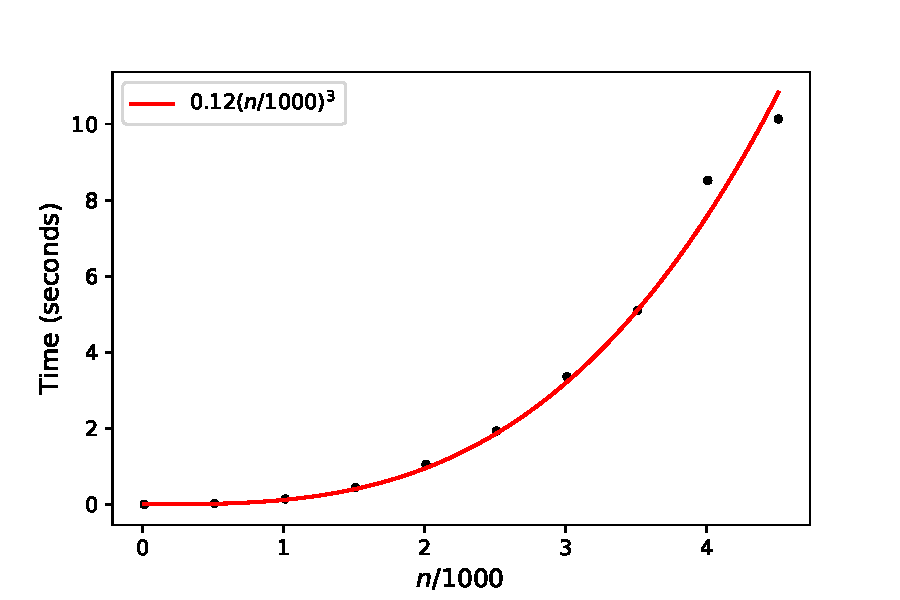
\includegraphics[scale=0.7]{images/lin_reg/inv_time.pdf}
\caption{How matrix inversion scales with dimension. Code used to generate this plot can be found \href{https://github.com/siavashaslanbeigi/ml_notes/blob/master/src/lin_reg/inv_time.ipynb}{\color{blue} here}.}
\label{linreg-fig:inv-time}
\end{figure}

If inverting $X^TX$ is not possible in practice, how else can we estimate the parameters $\theta$? Remember we obtained the normal equation by minimizing the cost function $J(\theta)$ (see \eqref{linreg-eq:multi-costfunc} or \eqref{linreg-eq:multi-costfunc-mat}). In the next section we will describe an algorithm, called Gradient Descent, which directly minimizes $J(\theta)$ and is faster for large values of $n$. How large is too large for the normal equation? About $n\simeq10,000$. That seems like an unreasonably large number of features. For instance, it's hard to imagine there could be $10,000$ features relevant for predicting house prices. Consider, though, making predictions based on images. If every pixel is considered a feature, which is often the case for image recognition problems, having $10,000$ features is equivalent to processing images that are only $100\text{px}\times100\text{px}$; not large by any means!


% Polynomial Regression --------------------------------
\subsection{Polynomial regression}
What if our data is better modeled as a polynomial? For instance, fitting a linear model to data shown in Figure \ref{linreg-fig:poly-data} doesn't seem appropriate. As it turns out, the following model provides a much better representation:
\begin{equation}
h_\theta(x) = \theta_0 + \theta_1 x + \theta_2 x^2 + \theta_3 x^3
\label{linreg-eq:poly-example}
\end{equation}
Can we use the machinery of linear regression to estimate the coefficients $\theta_0\dots\theta_3$? Consider the following definitions:
\begin{equation}
    x_1 = x, \qquad x_2 = x^2, \qquad x_3 = x^3.
\end{equation}
using which \eqref{linreg-eq:poly-example} takes the form \eqref{linreg-eq:multi-hypothesis}, or equivalently \eqref{linreg-eq:multi-hypothesis-mat} where the feature vector is given by:
\begin{equation*}
    \begin{pmatrix}
        1 \\
        x \\
        x^2 \\
        x^3
    \end{pmatrix}.
\end{equation*}
By transforming non-linear terms into new features, we can carry out linear regression as prescribed in the previous section. This trick can be used for far more complicated models, such as
\begin{equation}
    h_{\theta}(x) = \theta_0 + \theta_1 x^2 e^{-2x} + \theta_2 \sqrt{x}.
\end{equation}
Given that we can treat such complicated functions, what's with the word \textit{linear} in linear regression? It refers to the parameters $\theta$. An example of a model that cannot be treated using linear regression is $h_{\theta}(x) = e^{-\theta x}$, because it's not a linear function of $\theta$.

\begin{figure}[ht]
\centering
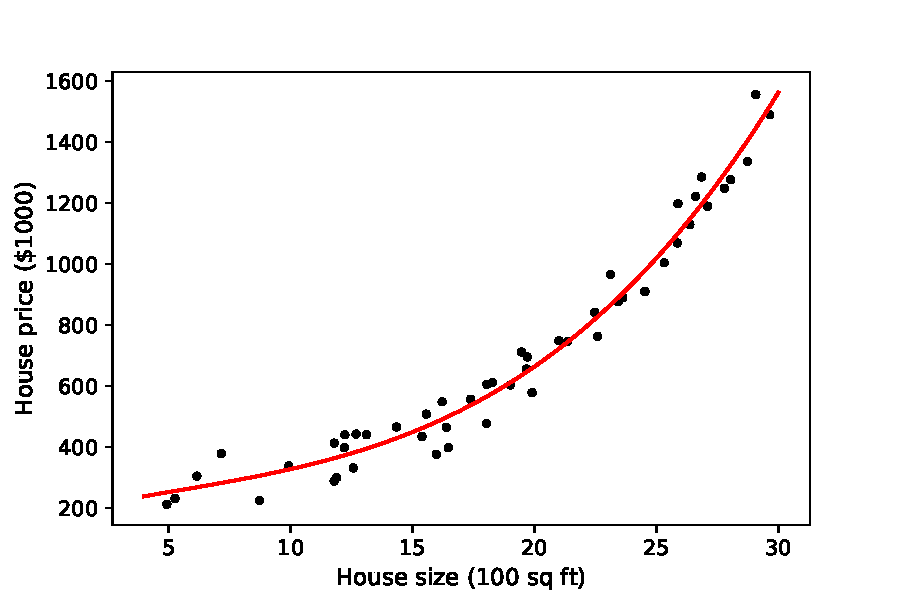
\includegraphics[scale=0.7]{images/lin_reg/poly-data.pdf}
\caption{Non-linear relationship between house price and size. Code used to generate this plot can be found \href{https://github.com/siavashaslanbeigi/ml_notes/blob/master/src/lin_reg/poly.ipynb}{\color{blue} here}.}
\label{linreg-fig:poly-data}
\end{figure}



% Probabilistic view -----------------------------------
\subsection{Probabilistic view}
Suppose we look at houses with similar characteristics such as number of bedrooms, number of floors, age, etc. Even though they are similar, they will likely not have the exact same price. For instance, one owner may be under time pressure and is willing to sell below market price. We should always expect a certain degree of randomness that our features cannot capture. We can, however, hope to design a model that makes the right predictions \textit{on average}. This suggests a probabilistic approach for modeling. For a given set of features $x$, we can think of the house price $y$ as a random variable with a certain probability distribution, whose mean is given by the hypothesis $h_{\theta}(x)$.

For simplicity, let's say $y$ has a normal distribution with standard deviation $\sigma$, and that all observations are independent. What is the probability of observing the training set $(x^{(1)}, y^{(1)}), \dots, (x^{(m)}, y^{(m)})$, assuming that our hypothesis $h_{\theta}(x)$ is correct on average? The probability that we observe a house with features $x^{(i)}$ and price $y^{(i)}$ is
\begin{equation}
    P^{(i)} = \frac{1}{\sqrt{2\pi\sigma^2}}\exp\left[-\frac{(y^{(i)} - h_{\theta}(x^{(i)}))^2}{2\sigma^2}\right].
\end{equation}
Since we're assuming all observations are independent, the probability of observing the training set is given by
\begin{equation}
    P = \prod_{i=1}^mP^{(i)} = \frac{1}{(2\pi\sigma^2)^{\frac{m}{2}}}\exp\left[-\sum_{i=1}^{m}\frac{(y^{(i)} - h_{\theta}(x^{(i)}))^2}{2\sigma^2}\right].
    \label{linreg-eq:mle-simple1}
\end{equation}
The quantity in the exponent can be rewritten in terms of $J(\theta)$
(see \eqref{linreg-eq:multi-costfunc}):
\begin{equation}
    P = \frac{1}{(2\pi\sigma^2)^{\frac{m}{2}}}\exp\left[-\frac{mJ(\theta)}{\sigma^2}\right].
    \label{linreg-eq:mle-simple2}
\end{equation}
Interesting! The probability of observing the training set can be written in terms of the cost function. In fact, the parameters $\theta$ that maximize the probability of observing the training set are precisely those that minimize the cost function $J(\theta)$. Picking the parameters of a model to maximize the probability of observing the dataset is called \textit{maximum likelihood estimation}. Before we picked the cost function based on heuristic arguments; now we see there's a deeper principle from which it can be arrived at.

Note that going from \eqref{linreg-eq:mle-simple1} to \eqref{linreg-eq:mle-simple2} assumes all observations are independent and have the same standard deviation $\sigma$. If every $y^{(i)}$ has its own standard deviation $\sigma_i$, the following cost function should be minimized:
\begin{equation}
    \tilde{J}(\theta) = \frac{1}{2m}\sum_{i=1}^{m}\frac{1}{\sigma_i^2}(h_{\theta}(x^{i}) - y^{(i)})^2.
\end{equation}
The wider the distribution of $y^{(i)}$ (i.e. the larger $\sigma_i$), the less it contributes to the overall cost. This makes sense: if $\sigma_i$ is very large compared to the other examples, we do not have much confidence in $y^{(i)}$, so we shouldn't assign too much weight to it.

We can further generalize to the case where $y^{(1)}, y^{(2)}, \dots, y^{(m)}$ are distributed as a multivariate Gaussian with covariance matrix $\Sigma$. Probability of observing the training set is then given by
\begin{equation}
    P = \frac{1}{(2\pi|\Sigma|)^{\frac{m}{2}}} e^{-m\tilde{J}(\theta)},
\end{equation}
where
\begin{align}
    \tilde{J} &= \frac{1}{2m}\sum_{i,i'=1}^{m}\Sigma^{-1}_{ii'}(y^{(i)} - h_{\theta}(x^{(i)}))(y^{(i')} - h_{\theta}(x^{(i')}))\notag\\
    &= \frac{1}{2m}\sum_{i,i'=1}^{m}\Sigma^{-1}_{ii'}[Y - X\theta]_i[Y - X\theta]_{i'}\notag\\
    &= \frac{1}{2m}(X\theta-Y)^T\Sigma^{-1}(X\theta-Y).
\end{align}
This expression is very similar to \eqref{linreg-eq:costfunc-mat}, except for the appearance of $\Sigma$. Again, maximizing $P$ is equivalent to minimizing $\tilde{J}$. Following the same steps as in section \ref{linreg-sec:normaleq}, it can be shown that
\begin{equation}
    \nabla_{\theta}\tilde{J}=\frac{1}{m}X^T\Sigma^{-1}(X\theta-Y).
\end{equation}
Setting $\nabla_{\theta}\tilde{J}$ to zero and solving for $\theta$:
\begin{equation}
    \theta = (X^T\Sigma^{-1}X)^{-1}X^T\Sigma^{-1}Y.
    \label{linreg-eq:costfunc-mat-err}
\end{equation}
Figure \ref{linreg-fig:yerror} shows an example of using \eqref{linreg-eq:costfunc-mat} vs. \eqref{linreg-eq:costfunc-mat-err} to fit house prices. When the training set is large, the difference is likely quite small because variation in the data captures the underlying distribution quite well. Indeed, we cannot know the distribution of $\{y^{(i)}\}$ in the first place if we don't collect a lot of data. In physical experiments, the distribution of $y^{(i)}$ depends largely on the measuring apparatus. No measurement is ever 100\% accurate and it is crucial to understand the noise.


\begin{figure}[ht]
\centering
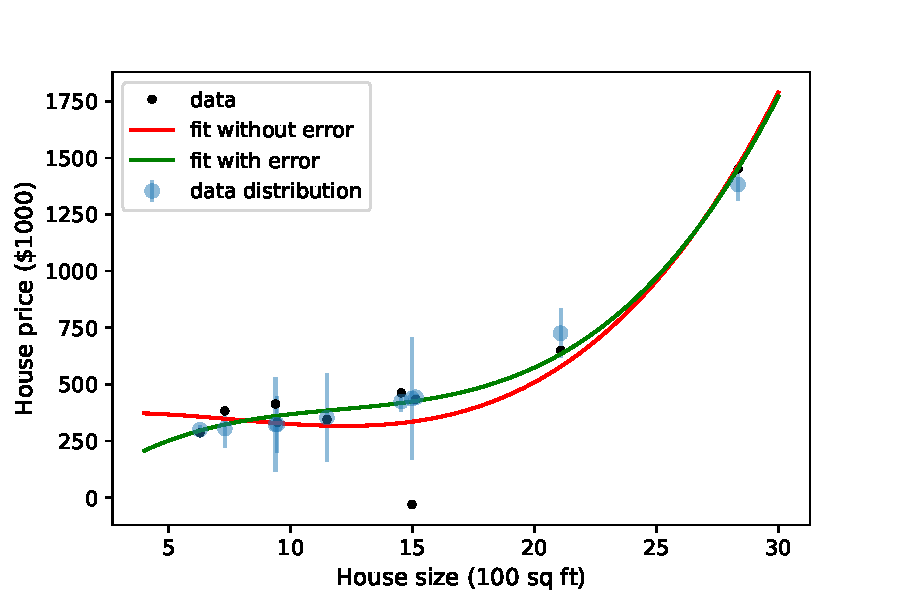
\includegraphics[scale=0.7]{images/lin_reg/yerror.pdf}
\caption{Fitting house prices when $y^{(i)}$ are drawn from different normal distributions. Blue dots show the mean of $y^{(i)}$ and the error bars show the standard deviation. Black dots are sampled house prices. The red fit uses \eqref{linreg-eq:costfunc-mat}, while the green fit uses \eqref{linreg-eq:costfunc-mat-err}. Code used to generate this plot can be found \href{https://github.com/siavashaslanbeigi/ml_notes/blob/master/src/lin_reg/yerror.ipynb}{\color{blue} here}.}
\label{linreg-fig:yerror}
\end{figure}


% Gradient Descent =====================================
\newpage
\section{Gradient Descent}
We saw in the previous section that training linear regression involves minimizing a cost function $J(\theta_1,\dots,\theta_N)$. We were able to carry out the minimization analytically and arrived at the normal equation. That is only possible because the hypothesis function $h_{\theta}(x)$ is linear in the fitting parameters $\theta_1,\dots,\theta_N$, which is not the case for most other learning algorithms.
Even for linear regression, as we explained in section \ref{section:normal-eq-infeasible}, the normal equation becomes infeasible when there are a large number of features. Therefore, we need an algorithm for minimizing a generic cost function $J(\theta_1,\dots,\theta_N)$. \textit{Gradient descent} is one such algorithm. To make the notation simpler, we will use $\theta$ to denote the vectors of parameters $\theta_1,\dots,\theta_N$ and simply write the cost function as $J(\theta)$.

The general idea of gradient descent is to start at some value of $\theta$, and then keep changing $\theta$ to reduce $J$ as much as possible, until we hopefully end up at the minimum. How do we change $\theta$? One way is to look for the direction along which $J$ decreases the fastest locally, and take a small step in that direction. This makes sense, since our goal is to minimize $J$ and we want to arrive at the minimum as quickly as possible. What \textit{is} the direction along which $J$ decreases the fastest? The answer turns out to be the opposite direction of the gradient $\nabla J$. To see why this makes sense, consider the Taylor expansion of $J$ about $\theta$:
\begin{equation}
    J(\theta + \delta\theta) =  J(\theta) + \nabla J \cdot \delta\theta + \cdots.
\end{equation}
If we make a small move in the opposite direction of the gradient, i.e. $\delta\theta = -\epsilon \nabla J$ where $\epsilon$ is a sufficiently small positive number, the cost function is guaranteed to decrease:
\begin{equation}
   \Delta J = J(\theta + \delta\theta) -  J(\theta) \approx -\epsilon \nabla J \cdot \nabla J < 0.
\end{equation}
This doesn't quite prove that $J$ decreases the \textit{fastest} in this direction. To see why that is, note that the first-order change in $J$ is given by the inner product of the vectors $\nabla J$ and $\delta \theta$: $\Delta J \approx \nabla J \cdot \delta\theta$. If we constrain the magnitude of $\delta \theta$, its inner product with $\nabla J$ is most negative when it is pointing in the opposite direction. A formal proof of this result is presented in Appendix \ref{app-section:gd}.

One step of gradient descent moves us along the direction of steepest descent as follows
\begin{equation}
    \theta := \theta - \alpha \nabla J,
\end{equation}
where $\alpha > 0$ is called the \textit{learning rate} and determines how long a step we take along the direction $-\nabla J$. Concretely, this is how gradient descent works:
\begin{enumerate}
    \item Start from some value $\theta^{(0)}$ and compute $\nabla J(\theta^{(0)})$.
    \item $\theta^{(1)}=\theta^{(0)}-\alpha\nabla J(\theta^{(0)})$.
    \item $\theta^{(2)}=\theta^{(1)}-\alpha\nabla J(\theta^{(1)})$.
    \item $\dots$
\end{enumerate}
Figure \ref{graddes-fig:gd2} demonstrates this using a simple cost function: $J(\theta)=\theta^2$. With an appropriate learning rate $\alpha=0.1$ and starting point $\theta^{(0)}=2$, gradient descent is able to find the minimum after about $20$ steps. It's a bit like rolling a ball down a valley; gravity will work its magic and the ball will eventually settle at the bottom. Note that even though the learning rate is constant, the steps keep getting smaller. The reason is that the closer to the minimum we get, the smaller the gradient becomes: at $\theta = 2$ we would take a step of size $-\alpha J'(2) = -0.4$, while at $\theta = 0.5$ the step size would only be $-0.1$.
\footnote{
The ball-rolling analogy breaks down here, since the ball speeds up as it gets to the bottom. In fact, the ball will oscillate about the minimum until it comes to a stop due to friction.
}


\begin{figure}[ht]
\centering
\includegraphics[scale=0.6]{images/grad_des/gd2.pdf}
\caption{Gradient descent applied to $J(\theta)=\theta^2$. The starting and end points are shown by red and green dots, respectively. Code used to generate this plot can be found \href{https://github.com/siavashaslanbeigi/ml_notes/blob/master/src/grad_des/basics.ipynb}{\color{blue} here}.}
\label{graddes-fig:gd2}
\end{figure}


% Impact of the learning rate --------------------------
\subsection{Impact of the learning rate}
Each step of gradient descent moves $\theta$ by $-\alpha\nabla J(\theta)$. If $\alpha$ is too small, each step will make little progress and gradient descent will take a long time to converge to the minimum. This is demonstrated in Figure \ref{graddes-fig:gd2-slow}, where the learning rate has been reduced $\alpha=0.02$.

On the other hand, if $\alpha$ is too large, gradient descent might not converge at all. This is demonstrated in Figure \ref{graddes-fig:gd2-overshoot}, where $\theta^{(0)}=0.5$ and $\alpha = 1.1$. The first step overshoots the minimum and ends up at $\theta=-0.6$, where the gradient is even higher. This keeps on repeating and the steps keep getting larger. Earlier we showed that moving in the opposite direction of $\nabla J$ should decrease $J$. Why, then, does $J$ increase in this example? The reason is that moving from $\theta$ to $\theta-\alpha\nabla J$ is only guaranteed to decrease $J$ if $J(\theta-\alpha\nabla J) \approx J(\theta) - \alpha\nabla J\cdot \nabla J$, for which $\alpha$ needs to be sufficiently small.

\begin{figure}[ht]
    \begin{subfigure}[ht]{\linewidth}
        \centering
        \includegraphics[scale=0.45]{images/grad_des/gd2_slow.pdf}
        \caption{If $\alpha$ is too small, gradient descent will take long to converge.}
        \label{graddes-fig:gd2-slow}
    \end{subfigure}%
    
    \begin{subfigure}[ht]{\linewidth}
        \centering
        \includegraphics[scale=0.45]{images/grad_des/gd2_overshoot.pdf}
        \caption{If $\alpha$ is too large, gradient descent might not converge.}
        \label{graddes-fig:gd2-overshoot}
    \end{subfigure}%
    
    \caption{Impact of the learning rate on convergence. The cost function used is $J(\theta)=\theta^2$. Code used to generate this plot can be found \href{https://github.com/siavashaslanbeigi/ml_notes/blob/master/src/grad_des/basics.ipynb}{\color{blue} here}.}
\end{figure}

It is hard to guess the appropriate learning rate \textit{a priori}. In general, a good way of checking if gradient descent is working is by plotting $J$ after every step.
With a sufficiently small value of $\alpha$, $J$ should decrease at every step. If it is increasing, we can try decreasing $\alpha$. If it is decreasing too slowly, we can try increasing $\alpha$.
Figure \ref{graddes-fig:gd2-progress} shows how $J(\theta)=\theta^2$ changes for gradient descent runs in Figures \ref{graddes-fig:gd2}, \ref{graddes-fig:gd2-slow}, and \ref{graddes-fig:gd2-overshoot}. In case of Figure \ref{graddes-fig:gd2}, $J$ converges to the minimum after about 10 iterations. For the run shown in Figure \ref{graddes-fig:gd2-overshoot}, $J$ increases after every step, which means the learning rate is too large.

This way of tracking the progress of gradient descent is easily generalizable when there are many features, i.e. when $J$ is a function of many variables. That's not the case for Figures such as \ref{graddes-fig:gd2}, where we plot $J$ as a function of $\theta$.

\begin{figure}[ht]
\centering
\includegraphics[scale=0.6]{images/grad_des/gd2_progress.pdf}
\caption{Tracking the progress of gradient descent applied to  $J(\theta)=\theta^2$. Code used to generate this plot can be found \href{https://github.com/siavashaslanbeigi/ml_notes/blob/master/src/grad_des/basics.ipynb}{\color{blue} here}.}
\label{graddes-fig:gd2-progress}
\end{figure}


% Local minima and initialization ----------------------
\subsection{Local minima and initialization}
Let's now look at a more complicated function:
\begin{equation}
   J(\theta) = \frac{12}{5} \theta^4 + \frac{4}{5} \theta^3 - \frac{18}{5} \theta^2 + 2.
   \label{graddes-eq:j4}
\end{equation}
It has a global minimum at $\theta=-1$, a local minimum at $\theta=+3/4$, and a local maximum at $\theta=0$. Will gradient descent always be able to find the global minimum? Unfortunately, no. It depends on the starting point. This is demonstrated in Figure \ref{graddes-fig:gd4-init}. For any starting point $\theta^{(0)}>0$, gradient descent will converge to the local minimum, while if $\theta^{(0)}<0$, it will find the global minimum.

\begin{figure}[ht]
    \begin{subfigure}{\linewidth}
        \centering
        \includegraphics[scale=0.45]{images/grad_des/gd4_local.pdf}
        \caption{Converging to the local minimum.}
        \label{graddes-fig:gd4-local}
    \end{subfigure}%
    
    \begin{subfigure}{\linewidth}
        \centering
        \includegraphics[scale=0.45]{images/grad_des/gd4_global.pdf}
        \caption{Converging to the global minimum.}
        \label{graddes-fig:gd4-global}
    \end{subfigure}%
    
    \caption{Impact of initialization on convergence. Cost function is given by \eqref{graddes-eq:j4}. Number of gradient descent steps in each case is 30. Code used to generate this plot can be found \href{https://github.com/siavashaslanbeigi/ml_notes/blob/master/src/grad_des/basics.ipynb}{\color{blue} here}.}
    \label{graddes-fig:gd4-init}
\end{figure}

Another interesting feature of \eqref{graddes-eq:j4} is that it has a local maximum at $\theta=0$. If we initialize gradient descent at $\theta=0$, it will not make any progress at all, since $J'(0)=0$. Even if we initialize close to the local maximum, progress will be slow, since $J'(\theta)$ is small there. Figure \ref{graddes-fig:gd4-slow} demonstrates this, where the learning rate is kept the same as that in Figure \ref{graddes-fig:gd4-init}, but the starting point is changed to $\theta=-0.01$ and the number of iterations is increased by a factor of 3. Even with so many more steps, gradient descent is not able to converge to the global minimum.


\begin{figure}[ht]
\centering
\includegraphics[scale=0.6]{images/grad_des/gd4_slow.pdf}
\caption{Gradient descent takes very small steps in regions where the gradient is small. Cost function is given by \eqref{graddes-eq:j4}. Code used to generate this plot can be found \href{https://github.com/siavashaslanbeigi/ml_notes/blob/master/src/grad_des/basics.ipynb}{\color{blue} here}.}
\label{graddes-fig:gd4-slow}
\end{figure}


% Feature scaling --------------------------------------
\subsection{Feature scaling}
So far we've been looking at 1d functions. Let's now look at a 2d example:
\begin{equation}
    J(\theta_1, \theta_2)=9(\theta_1 - 2)^2+(\theta_2 - 1)^2.
    \label{graddes-eq:fs}
\end{equation}
Its minimum occurs at
\begin{equation*}
   \theta=\begin{pmatrix}\theta_1\\\theta_2\end{pmatrix}=\begin{pmatrix}2\\1\end{pmatrix},
\end{equation*}
and its gradient is given by
\begin{equation*}
    \nabla J = \begin{pmatrix}18(\theta_1-2)\\2(\theta_2-1)\end{pmatrix},
\end{equation*}
so the gradient descent update rule is
\begin{equation*}
   \begin{pmatrix}\theta_1\\\theta_2\end{pmatrix} := \begin{pmatrix}\theta_1\\\theta_2\end{pmatrix} - \alpha\begin{pmatrix}18(\theta_1-2)\\2(\theta_2-1)\end{pmatrix}.
\end{equation*}
In Figure \ref{graddes-fig:fs-zz}, we've applied gradient descent to \eqref{graddes-eq:fs}, with $\alpha=0.1$ and starting point $\theta_1=\theta_2=5$. It makes large zig-zag moves about $\theta_1=2$ and approaches the minimum slowly along the $\theta_2$ direction. The reason is that the gradient in the $\theta_1$ direction is much larger. This can be seen from the contours of $J$; they are elongated vertically. The first step, for instance, goes from $\begin{pmatrix}5\\5\end{pmatrix}$ to $\begin{pmatrix}-0.4\\4.2\end{pmatrix}$, decreasing $\theta_1$ by $5.4$ and $\theta_2$ by only $0.8$.

One way to avoid the zig-zag moves is to reduce $\alpha$, so that we do not overshoot $\theta_1=2$. This is done in Figure \ref{graddes-fig:fs-zz-fixed}, where $\alpha=0.05$. Gradient descent takes one big step along the $\theta_1$ direction, and many smaller ones along $\theta_2$ towards the minimum. Since we decreased $\alpha$ to avoid large moves in the $\theta_1$ direction, steps along $\theta_2$ are now much smaller than they need to be.


\begin{figure}[ht]
    \begin{subfigure}{\linewidth}
        \centering
        \includegraphics[scale=0.45]{images/grad_des/fs_zigzag.pdf}
        \caption{$\alpha=0.1$.}
        \label{graddes-fig:fs-zz}
    \end{subfigure}%
    
    \begin{subfigure}{\linewidth}
        \centering
        \includegraphics[scale=0.45]{images/grad_des/fs_zigzag_fixed.pdf}
        \caption{$\alpha=0.05$.}
        \label{graddes-fig:fs-zz-fixed}
    \end{subfigure}%
    
    \caption{Gradient descent applied to \eqref{graddes-eq:fs}. The starting point is $\theta_1=\theta_2=5$ and the first $10$ steps are shown. Code used to generate this plot can be found \href{https://github.com/siavashaslanbeigi/ml_notes/blob/master/src/grad_des/feature_scaling.ipynb}{\color{blue} here}.}
    \label{graddes-fig:fs-issues}
\end{figure}

The problem we're facing is that $J$ has a much larger gradient along $\theta_1$ than $\theta_2$. As it turns out, we can get around this issue by a simple redefinition:
\begin{equation}
    \tilde{\theta}_1 = 3(\theta_1-2), \qquad
    \tilde{\theta}_2 = \theta_2-1,
    \label{graddes-eq:fs-rescaling}
\end{equation}
so that $J=\tilde{\theta}_1^2 + \tilde{\theta}_2^2$. We can now use gradient descent to minimize $J$ w.r.t $\tilde{\theta}_1$ and $\tilde{\theta}_2$, and then simply use \eqref{graddes-eq:fs-rescaling} to find the minimum w.r.t $\theta$.
\footnote{
Since $J$ is simple enough, we can check this analytically. The minimum of $\tilde{\theta}_1^2 + \tilde{\theta}_2^2$ occurs at $\tilde{\theta}_1=\tilde{\theta}_2=0$, and with the rescaling \eqref{graddes-eq:fs-rescaling}, we recover the original minimum: $\theta_1 = \tilde{\theta}_2/3+2=2$, $\theta_2 = \tilde{\theta}_1+1=1$.
}
The crucial point is that the gradient of $J$ along $\tilde{\theta}_1$ and $\tilde{\theta}_2$ is the same, so gradient descent can now move directly towards the minimum. This is demonstrated in Figure \ref{graddes-fig:fs-scaled}. Contours of $J$ w.r.t $\tilde{\theta}_1$ and $\tilde{\theta}_2$ are circular, and we can now use a larger learning rate ($\alpha=0.2$) to get much closer to the minimum after the same number of steps.


\begin{figure}[ht]
\centering
\includegraphics[scale=0.6]{images/grad_des/fs_scaled.pdf}
\caption{Gradient descent applied to $\theta_1^2+\theta_2^2$, with $\alpha=0.2$ and starting point $\theta_1=\theta_2=5$. The first $10$ steps are shown. Code used to generate this plot can be found \href{https://github.com/siavashaslanbeigi/ml_notes/blob/master/src/grad_des/feature_scaling.ipynb}{\color{blue} here}.}
\label{graddes-fig:fs-scaled}
\end{figure}

Let's consider the implications of what we have just seen for linear regression. Suppose we are considering two features for predicting house prices: size of house $x_1$ ($\text{ft}^2)$ and number of bedrooms $x_2$. The hypothesis function $h$ and cost function $J$ are given as usual:
\begin{equation}
    h_{\theta}(x)=\theta_0+\theta_1x_1+\theta_2x_2, \qquad
    J=\frac{1}{2m}\sum_{i=1}^{m}(\theta_0+\theta_1x^{(i)}_1+\theta_2x^{(i)}_2-y^{(i)})^2.
\end{equation}
A reasonable range of values for these features is $x_1\sim 100-1000$ and $x_2\sim 1-10$. Because $x_1$ is much larger than $x_2$, $J$ changes a lot more quickly along $\theta_1$ than $\theta_2$. We just saw that running gradient descent on functions like this is terribly inefficient, because it will spend most of the time zig-zagging in the $\theta_1$ direction. Again, we can get around this problem by a redefinition
\begin{equation}
    \tilde{x}_1 = \frac{x_1 - \mu_1}{\sigma_1}, \qquad
    \tilde{x}_2 = \frac{x_2 - \mu_2}{\sigma_2}
    \label{graddes-eq:fs-linreg}
\end{equation}
where
\begin{equation}
    \mu_j = \frac{1}{m}\sum_{i=1}^{m}x^{(i)}_j, \qquad
    \sigma_j = \frac{1}{m}\sum_{i=1}^{m}(x^{(i)}_j-\mu_j)^2.
\end{equation}
We are subtracting the mean $\mu_j$ of every feature $x_j$ in the training set and scaling it by the standard deviation $\sigma_j$. As a result, the new features $\tilde{x}_1$ and $\tilde{x}_2$ take on values in a similar range (in most cases somewhere between $-3$ and $3$). This procedure is called \textit{feature scaling}. There are other ways of transforming the original features so they take on similar values. For instance, instead of dividing $x_j - \mu_j$ by the standard deviation $\sigma_j$, we could divide by the range of $x_j$, i.e. $r_j=\text{max}(x_j)-\text{min}(x_j)$.

We can now run linear regression on the normalized features. Concretely, we will consider the hypothesis function
\begin{equation}
    h=\tilde{\theta}_0+\tilde{\theta}_1\tilde{x}_1+\tilde{\theta}_2\tilde{x}_2,
    \label{graddes-eq:fs-linreg-hyp}
\end{equation}
and minimize the following cost function for $\tilde{\theta}_0, \tilde{\theta}_1$, and $\tilde{\theta}_2$:
\begin{equation}
    J=\frac{1}{2m}\sum_{i=1}^{m}(\tilde{\theta}_0+\tilde{\theta}_1\tilde{x}^{(i)}_1+\tilde{\theta}^{(i)}_2\tilde{x}^{(i)}_2-y^{(i)})^2.
\end{equation}
Gradient descent we will not zig-zag along $\tilde{\theta}_1$, since $\frac{\partial J}{\partial\tilde{\theta}_1}$ is not much larger than $\frac{\partial J}{\partial\tilde{\theta}_2}$. (Contours of $J$ w.r.t $\tilde{\theta}_1$ and $\tilde{\theta}_1$ should be more or less circular.)

After finding the optimal parameters $\tilde{\theta}$ using gradient descent, we can predict the price of an unseen house $x$ by following two steps: (i) transform $x$ to $\tilde{x}$ via \eqref{graddes-eq:fs-linreg}, (ii) plug $\tilde{x}$ in \eqref{graddes-eq:fs-linreg-hyp} to predict the house price. In other words:
\begin{equation}
    h(x)=\tilde{\theta}_0+\tilde{\theta}_1\frac{x_1 - \mu_1}{\sigma_1}+\tilde{\theta}_2\frac{x_2 - \mu_2}{\sigma_2}.
\end{equation}
Had we optimized using the original features $x$, we would find that
\begin{equation*}
    \theta_0 =\tilde{\theta}_0-\frac{\mu_1}{\sigma_1}\tilde{\theta}_1-\frac{\mu_2}{\sigma_2}\tilde{\theta}_2, \qquad
    \theta_1 = \frac{\tilde{\theta}_1}{\sigma_1}, \qquad
    \theta_2 = \frac{\tilde{\theta}_2}{\sigma_2}.
\end{equation*}
It is important to include the bias term when using feature scaling. Try the following experiment: ignore $\theta_0$ and $\tilde{\theta}_0$ in the analysis above, run linear regression once on the original features to find the optimal $\theta$, and once on the normalized features to find $\tilde{\theta}$. Then consider a new house $x$ and predict its price once using $\theta_1x_2+\theta_2x_2$, and another time using $\tilde{\theta}_1(x_1 - \mu_1)/\sigma_1+\tilde{\theta}_2(x_2 - \mu_2)/\sigma_2$. You will find that the answers are different. Can you see what went wrong?

% Gradient descent for linear regression ---------------
\subsection{Gradient descent for linear regression}
The gradient descent update rule for linear regression is given by (see \eqref{linreg-eq:costfunc-nbala})
\begin{equation}
    \theta := \theta - \frac{\alpha}{m}X^T(X\theta - Y),
\end{equation}
or equivalently (see \eqref{linreg-eq:costfunc-mat})
\begin{equation}
    \theta := \theta - \frac{\alpha}{m}\sum_{i=1}^{m}(\theta^Tx^{(i)} - y^{(i)})x^{(i)}.
\end{equation}


% Line search ------------------------------------------
\subsection{Line search}
We've seen so far that picking the learning rate is quite tricky. If it's too large, gradient descent might not converge. If it's too small, convergence might be very slow. Is there a way of automatically picking the optimal learning rate? Let's remember what the learning rate is actually doing. One step of gradient descent moves us in the direction $-\nabla J$ by $\alpha\nabla J$: $\theta \to \theta - \alpha \nabla J(\theta)$. So $\alpha$ determines how long a step we take in the direction $-\nabla J$. How about, then, tuning $\alpha$ to reduce $J$ as much as possible along the direction $-\nabla J$? After all, our goal is to minimize $J$! What exactly would this involve? We can start with one value of $\alpha$, move to $\theta - \alpha \nabla J(\theta)$, and compute the value of the cost function there: $J(\theta - \alpha \nabla J(\theta))$. We can repeat this for all possible values of $\alpha$ and ultimately pick the value that minimizes $J(\theta - \alpha \nabla J(\theta))$. This means we need to minimize the $1$-dimensional function
\begin{equation}
    f(\alpha) = J(\theta - \alpha \nabla J(\theta))
\end{equation}
at every step of gradient descent. Solving for $f'(\alpha)=0$, we find
\begin{equation}
    \frac{df}{d\alpha} =-\nabla J|_{\theta}\cdot \nabla J|_{\theta - \alpha \nabla J} = 0.
    \label{graddes-eq:opt1}
\end{equation}
I have used the notation $\nabla J|_{\theta}$ to explicitly state where the gradient is being valued. This equation is telling us that the optimal learning rate moves us to a point where the gradient vector is  orthogonal to the one at the current step. In other words, the inner product between $\nabla J|_{\theta}$ and $\nabla J|_{\theta - \alpha \nabla J}$ is zero. Assuming $\nabla J|_{\theta}\neq 0$ (so we're not sitting on a local optimum), this implies that $J|_{\theta - \alpha \nabla J}$ should either be zero, meaning we've reached a (local) minimum, or it should be orthogonal to $\nabla J|_{\theta}$.

In general, we will need to carry out this optimization numerically. In the special case where $J$ is a quadratic function of $\theta$, however, this can be done analytically. Consider the cost function
\begin{equation}
    J(\theta) = \frac{1}{2}\theta^TA\theta + \theta^TB + C,
\end{equation}
where $A$ is an $N\times N$ positive-definite matrix, $B$ is an $N$-dimensional vector, and $C$ is a number. This describes an $N$-dimensional paraboloid. The cost function for linear regression takes precisely this form. Comparing this equation to \eqref{linreg-eq:multi-costfunc-mat}: $A=\frac{1}{m}X^TX$, $B=-\frac{1}{m}X^TY$, and $C=\frac{1}{m}Y^TY$. Since $J$ is quadratic in $\theta$, $\nabla J$ is linear:
\begin{equation}
    \nabla J = A\theta + B.
\end{equation}
Using this, it can be checked that
\begin{equation}
    \nabla J|_{\theta - \alpha \nabla J} = \nabla J|_{\theta} - \alpha A\nabla J|_{\theta}.
\end{equation}
We can now solve \eqref{graddes-eq:opt1} for the optimal learning rate:
\begin{equation}
    \alpha
        = \frac{(\nabla J)^T\nabla J}{(\nabla J)^TA(\nabla J)}
        = \frac{(A\theta + B)^T(A\theta + B)}{(A\theta + B)^TA(A\theta + B)}.
    \label{graddes-eq:opt-alpha}
\end{equation}

Let's look at what this optimal learning does for us in some special cases. Suppose $J$ is one-dimensional ($N=1$), so that $A$ and $B$ are numbers. The optimal learning rate is simply $\alpha=1/A$. The first step of gradient descent will take us from $\theta$ to $\theta - \alpha J'(\theta) = \theta - \frac{1}{A}(A\theta+B) = -B/A$, which is precisely where the global minimum is! No matter where we start, gradient descent will take us directly to the minimum in just one step, if we use the optimal learning rate. Consider now another case, where $J=\theta_1^2+\theta_2^3+\cdots+\theta_N^2$, i.e. $A=1_N$, $B=0$, and $C=0$. The optimal learning rate is $\alpha=1$. The first step of gradient descent takes us from $\theta$ to $\theta - \alpha (A\theta+B)=0$, which is the global minimum. Again, it only takes one step to find the minimum.

More generally, if $\nabla J$ is along the direction of an eigenvector of $A$, it will only take one step to get to the minimum. To see why, let $v$ be a normalized eigenvector of $A$ with eigenvalue $\lambda$: $Av=\lambda v$, $v^Tv=1$. If $\nabla J$ points along the direction of $v$, then $\nabla J = ||\nabla J|| v$ and $A(\nabla J)=\lambda ||\nabla J|| v = \lambda \nabla J$. Plugging this back in \eqref{graddes-eq:opt-alpha} we find $\alpha=1/\lambda$. One step of gradient descent would take us from $\theta$ to $\theta^{new} = \theta-\alpha\nabla J=\theta-\frac{1}{\lambda}\nabla J$. The gradient at $\theta^{new}$ is given by $A\theta^{new}+B=A\theta-\frac{1}{\lambda}A\nabla J+B=A\theta-\nabla J+B=0$, which means $\theta^{new}$ is the minimum.







\clearpage
\appendix
% Linear Algebra =======================================
\section{Linear Algebra}
Here we present definitions and proofs of most linear algebra results used in the notes.
\begin{definition}
The conjugate transpose $A^*$ of an $m\times n$ complex matrix $A$ is an $n \times m$ matrix defined as follows: $A^*_{ij}=\overline{A_{ji}}$. In other words, $A^*$ is obtained by first transposing $A$, and then take taking the complex conjugate of every entry, as shown in the example below:
\begin{equation}
    A =
    \begin{pmatrix}
        1 & 1+i & 2i \\
        3+2i & 2 & 5 \\
    \end{pmatrix},
    \qquad
    A^* =
    \begin{pmatrix}
        1 & 3-2i \\
        1-i & 2 \\
        -2i & 5 \\
    \end{pmatrix}.
\end{equation}
\end{definition}

\begin{definition}
A square complex matrix $A$ is called Hermitian matrix if it is equal to its conjugate transpose $A=A^*$. The following is an example of an Hermitian matrix:
\begin{equation}
    A =
    \begin{pmatrix}
        1 & 1+i \\
        1-i & 1 \\
    \end{pmatrix}.
\end{equation}
Note that a real Hermitian matrix is symmetric.
\end{definition}

\begin{theorem}
Eigenvalues of a Hermitian matrix are real.
\end{theorem}
 
\begin{proof}
Let $A$ be a Hermitian matrix and consider its eigenvalues and eigenvectors:
\begin{equation}
    Av_n=\lambda_nv_n.
\end{equation}
Applying $v_n^*$ to both sides:
\begin{equation}
    \lambda_n |v_n|^2 = v_n^*Av_n = v_n^*A^*v_n = (Av_n)^*v_n = (\lambda_nv_n)^*v_n = \overline{\lambda_n}|v_n|^2
    \label{appendix-eq:eig}
\end{equation}
where $|v_n|^2=v_n^*v_n>0$. Therefore, $\lambda_n=\overline{\lambda_n}$, which means $\lambda_n$ is real.
\end{proof}

\begin{theorem}
Eigenvectors of a Hermitian matrix $A$ with different eigenvalues are orthogonal, i.e.
\begin{equation}
    \lambda_n\ne\lambda_m \to v_n^*v_m=0.
\end{equation}
\end{theorem}

\begin{proof}
\begin{equation}
    \lambda_mv_n^*v_m = v_n^*(\lambda_mv_m) = v_n^*Av_m = v_n^*A^*v_m = (Av_n)^*v_m = \lambda_nv_n^*v_m,
\end{equation}
where the last one uses the fact that $\lambda_n$ is real. Thus, we've shown $(\lambda_m - \lambda_n)v_n^*v_m = 0$, and since we're assuming $\lambda_n\ne\lambda_m$, it follows that $v_n^*v_m=0$.
\end{proof}

\begin{definition}
\label{linalg-def:pos-def}
A Hermitian matrix $A$ is called \textit{positive definite} if it satisfies the following condition for all vectors $v$:
\begin{equation}
    v^*Av > 0.
\end{equation}
Note that $v^*Av$ is real, because $A$ is Hermitian: $\overline{v^*Av}=(v^*Av)^*=v^*A^*v=v^*Av$. Similarly, $A$ is called positive \textit{semi}-definite if $v^*Av$ is positive or zero: $v^*Av \ge 0$.
\end{definition}

\begin{theorem}
\label{linalg-def:pos-def-eig}
All eigenvalues of a positive-definite matrix are positive. Similarly, all eigenvalues of a positive semi-definite matrix are non-negative.
\end{theorem}

\begin{proof}
Let $A$ be a positive definite matrix and consider its eigenvalues and eigenvectors:
\begin{equation}
    Av_n=\lambda_nv_n.
\end{equation}
Applying $v^*$ t both sides: $\lambda_nv_n^*v_n=v_n^*Av_n > 0$, which implies $\lambda_n > 0$ since $v_n^*v_n>0$. The same argument shows that any non-zero eigenvalue of a positive semi-definite matrix is positive.
\end{proof}

% Singular-Value Decomposition =========================
\section{Singular-Value Decomposition}
\label{section:svd}
The singular-value decomposition (SVD) is a powerful result that applies to any matrix. In this section, we will derive the SVD and explain what it means intuitively. The SVD states that any $m\times n$ matrix $M$ can be written as
\begin{equation}
    M=UDV^T,
\end{equation}
where
\begin{itemize}
    \item $U$ is an $m\times m$ unitary matrix, i.e. it satisfies $U^TU=UU^T=1_m$, where $1_m$ is the $m$-dimensional identity matrix.
    \item $V$ is an $n\times n$ unitary matrix, i.e. satisfies $V^TV=VV^T=1_n$, where $1_n$ is the $n$-dimensional identity matrix.
    \item $D$ is an $m\times n$ matrix with zero elements everywhere except $D_{ii}\ge0$ where $i=1,\dots,\text{min}(m, n)$. So $D$ is diagonal and has at most $\text{min}(m, n)$ elements on the diagonal. These elements are called the singular values of $X$.
\end{itemize}

\subsection{Intuition}
Before delving into the proof, let's go through a simple example to understand what the matrices $V$, $D$, and $U$ are doing. Consider the following matrix
\begin{equation}
    M = \frac{1}{2}
    \begin{pmatrix}
        -\sqrt{3} & 3 \\
        5 & -\sqrt{3} \\
    \end{pmatrix},
\end{equation}
which admits the SVD
\begin{equation}
    U = \frac{1}{2}
    \begin{pmatrix}
        -1 & \sqrt{3} \\
        \sqrt{3} & 1 \\
    \end{pmatrix}, \qquad
    D =
    \begin{pmatrix}
        3 & 0 \\
        0 & 1 \\
    \end{pmatrix}, \qquad
    V = \frac{1}{2}
    \begin{pmatrix}
        \sqrt{3} & 1 \\
        -1 & \sqrt{3} \\
    \end{pmatrix}.
\end{equation}
Let's look at the action of $V^T$ on unit vectors $u_x$ and $u_y$. This is shown in Figure \ref{linalg-fig:svd-v}. It rotates the two vectors counterclockwise by $\pi/6$. We shouldn't be surprised that $V^T$ is acting as a rotation, since it is unitary. Let's remember why this is. A unitary matrix $A$ preserves inner products between vectors:
\begin{equation}
    (Av_1)^T(Av_2) = v_1^T(A^TA)v_2 = v_1^Tv_2.
\end{equation}
This means the angle between $v_1$ and $v_2$ is the same as that between $Av_1$ and $Av_2$. It also means that the norm of $v_1$ and $v_2$ remain unchanged under the action of $A$. Rotations and reflections have these properties.
Figure \ref{linalg-fig:svd-d} shows the application of $D$, after $V^T$ has been applied. We see that the vectors are being stretched ($D_{11}=3$) times along the $x$-axis, and remain unchanged along the $y$-axis, because $D_{22}=1$.
Finally, Figure \ref{linalg-fig:svd-u} shows the application of $U$ after $DV^T$ has been applied. The vectors are being reflected along the line that makes $\pi/3$ angle with the $x$-axis. Note that $UDV^Tu_x$ and $UDV^Tu_y$ are the first and second columns of $M$, respectively.

\begin{figure}[ht]
    \centering 
    \begin{subfigure}[ht]{\linewidth}
        \centering
        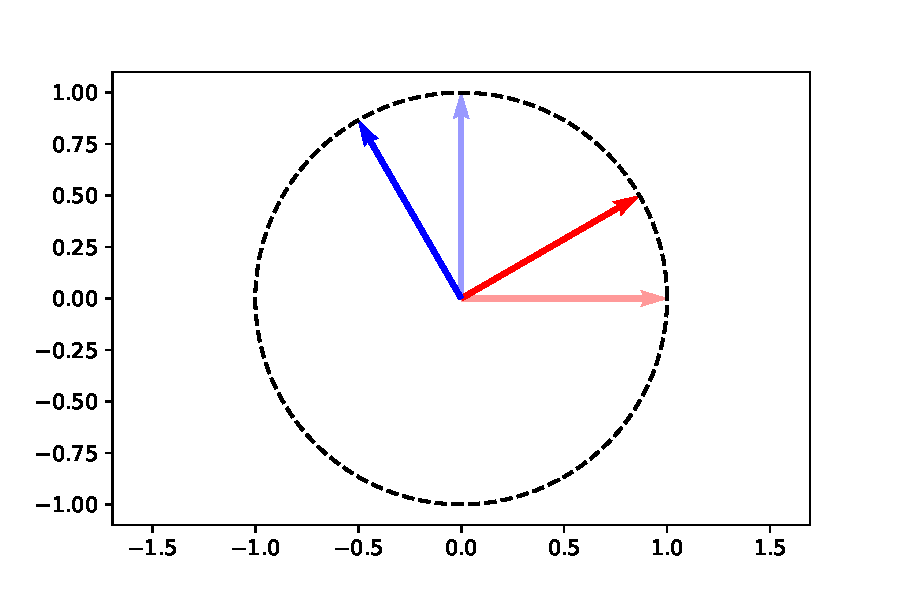
\includegraphics[scale=0.45]{images/lin_alg/svd_v.pdf}
        \caption{First step: applying $V^T$ to unit vectors $u_x$ (light red) and $u_y$ (light blue). $V^Tu_x$ and $V^Tu_y$ are the darker red and blue arrows, respectively.}
        \label{linalg-fig:svd-v}
    \end{subfigure}%
    
    \begin{subfigure}[ht]{\linewidth}
        \centering
        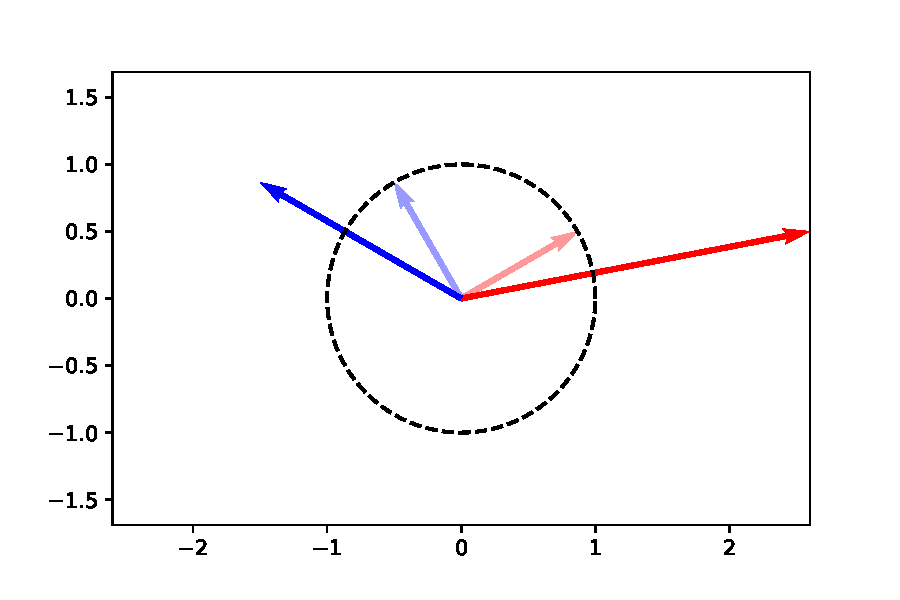
\includegraphics[scale=0.45]{images/lin_alg/svd_d.pdf}
        \caption{Second step: applying $D$ to $V^Tu_x$ (light red) and $V^Tu_y$ (light blue). $DV^Tu_x$ and $DV^Tu_y$ are the darker red and blue arrows, respectively.}
        \label{linalg-fig:svd-d}
    \end{subfigure}%
    
    \begin{subfigure}[ht]{\linewidth}
        \centering
        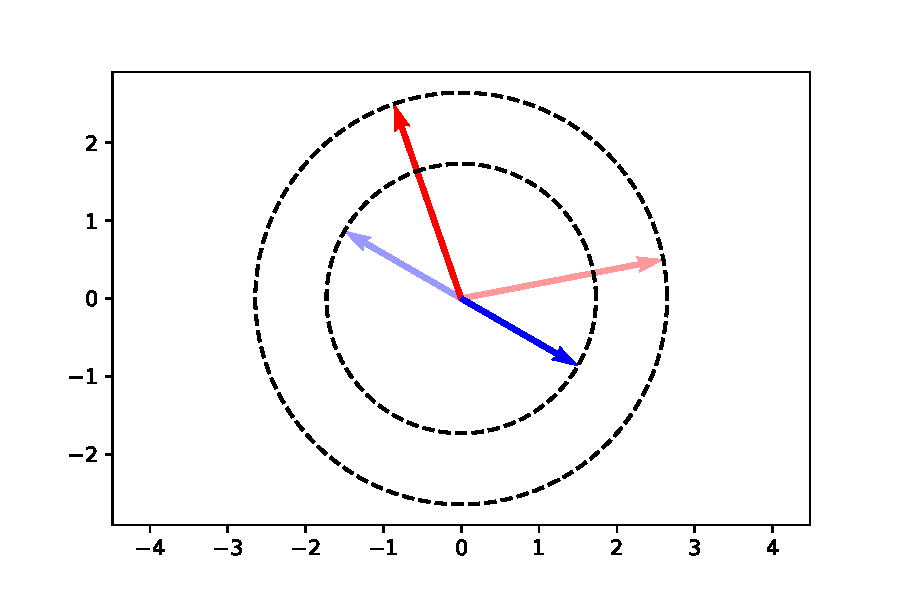
\includegraphics[scale=0.45]{images/lin_alg/svd_u.pdf}
        \caption{Third step: applying $U$ to to $DV^Tu_x$ (light red) and $DV^Tu_y$ (light blue). $UDV^Tu_x$ and $UDV^Tu_y$ are the darker red and blue arrows, respectively.}
        \label{linalg-fig:svd-u}
    \end{subfigure}
    \caption{Applying SVD of $M$ step by step. Code used to generate this plot can be found \href{https://github.com/siavashaslanbeigi/ml_notes/blob/master/src/lin_alg/svd.ipynb}{\color{blue} here}.}
    \label{linalg-fig:svd}
\end{figure}

SVD is telling us that any matrix can be decomposed into a rotation/reflection, scaling along the coordinate axes, and another rotation/reflection. This result applies even when $M$ is not a square matrix. For instance, if $M$ is $2\times3$: $V^T$ is a rotation/reflection in $\mathbb{R}^3$, $D$ projects the resulting vector into $\mathbb{R}^2$ and stretches it along the coordinate axes, and $U$ applies a final rotation/reflection in $\mathbb{R}^2$.


\subsection{Proof}
Let's now prove the singular-value decomposition. Consider the following two matrices
\begin{equation}
    \Sigma = M^TM, \qquad W = MM^T.
\end{equation}
Note that $\Sigma$ is $n\times n$, $W$ is $m\times m$, and they are both symmetric and positive semi-definite (see \ref{linalg-def:pos-def}):
\begin{align*}
    v^T\Sigma v &= v^TM^TMv = (Mv)^T(Mv) = \lVert Mv \rVert^2 \ge 0,\\
    v^TWv &= v^TMM^Tv = (M^Tv)^T(M^Tv) = \lVert M^Tv \rVert^2 \ge 0.
\end{align*}
Therefore, they can be diagonalized and all of their eigenvalues are non-negative (see \ref{linalg-def:pos-def-eig}):
\begin{equation}
    \Sigma v^{(i)} = \lambda_i v^{(i)}, \qquad
    (v^{(i)})^T v^{(j)} = \delta_{ij}, \qquad
    \lambda_i \ge 0
\end{equation}
where $i,j=1,\dots n$ and similarly for $W$:
\begin{equation}
    W v^{(i)} = \xi_i w^{(i)}, \qquad
    (w^{(i)})^T w^{(j)} = \delta_{ij}, \qquad
    \xi_i \ge 0,
\end{equation}
where $i,j=1,\dots m$.

The following results show that the eigenvalues and eigenvectors of $\Sigma$ and $W$ are closely related.

\begin{lemma}
\label{svd-lemma:mv}
When $\lambda_i > 0$, $Mv^{(i)}$ is an eigenvector of $W$ with eigenvalue $\lambda_i$. Also $\lVert Mv^{(i)} \rVert^2 =  \lambda_i$.
\end{lemma}
\begin{proof}
\begin{equation}
    W(Mv^{(i)}) = MM^TMv^{(i)} =M\Sigma v^{(i)} = M(\lambda_iv^{(i)}) = \lambda_i(Mv^{(i)}).
\end{equation}
Consider now the norm of $Mv^{(i)}$:
\begin{equation}
    (Mv^{(i)})^T(Mv^{(i)}) = (v^{(i)})^TM^TMv^{(i)} = (v^{(i)})^T\Sigma v^{(i)} = \lambda_i.
\end{equation}
Note that when $\lambda_i=0$, the norm of $Mv^{(i)}$ is zero, which means $Mv^{(i)}$ is the zero vector.
\end{proof}

\begin{lemma}
\label{svd-lemma:mtw}
When $\xi_i > 0$, $M^Tw^{(i)}$ is an eigenvector of $\Sigma$ with eigenvalue $\xi_i$. Also $\lVert M^Tw^{(i)} \rVert^2 =  \xi_i$.
\end{lemma}
\begin{proof}
\begin{equation}
    \Sigma(M^Tw^{(i)}) = M^T MM^T w^{(i)} =M^T W w^{(i)} = M^T(\xi_iw^{(i)}) = \xi_i(M^Tw^{(i)}).
\end{equation}
Consider now the norm of $M^Tw^{(i)}$:
\begin{equation}
    (M^Tw^{(i)})^T(M^Tw^{(i)}) = (w^{(i)})^TMM^Tw^{(i)} = (w^{(i)})^TW w^{(i)} = \xi_i.
\end{equation}
Note that when $\xi_i=0$, the norm of $M^Tw^{(i)}$ is zero, which means $M^Tw^{(i)}$ is the zero vector.
\end{proof}

\begin{corollary}
$\Sigma$ and $W$ share the same set of non-zero eigenvalues, of which there are at most $\text{min}(m, n)$.
\end{corollary}
\begin{proof}
Every non-zero eigenvalue of $\Sigma$ is also an eigenvalue of $W$ (see \ref{svd-lemma:mv}). But can $W$ have more non-zero eigenvalues than $\Sigma$? No, because every non-zero eigenvalue of $W$ is also an eigenvalue of $\Sigma$ (see \ref{svd-lemma:mtw}). Since $\Sigma$ and $W$ share the same set of non-zero eigenvalues, there cannot be more than $\text{min}(m, n)$ of them. For instance, if $m=2$ and $n=3$, $W$ can have at most two non-zero eigenvalues (because it's $2\times2$), and since $\Sigma$ cannot have more non-zero eigenvalues than $W$, it is guaranteed to have at least one zero eigenvalue, which means it is not invertible. 
\end{proof}

Let $\lambda_1,\dots,\lambda_k$ ($k\le \text{min}(m, n)$) denote the strictly positive eigenvalues of $\Sigma$ and $W$. Also let $v^{(1)},\dots,v^{(k)}$ be the corresponding eigenvectors of $\Sigma$, and $w^{(1)},\dots,w^{(k)}$ those of $W$. It follows from \ref{svd-lemma:mv} that
\begin{equation}
    w^{(i)} = \frac{1}{\sqrt{\lambda_i}}Mv^{(i)} \qquad i=1,\dots,k.
    \label{svd-eq:w}
\end{equation}
Let $v^{(k+1)},\dots,v^{(n)}$ and $w^{(k+1)},\dots,w^{(m)}$ be orthonormal eigenvectors corresponding to zero eigenvalues of $\Sigma$ and $W$, respectively. Now we define $V$, $D$, and $U$ as follows
\begin{align*}
    V_{ij} &= v^{(j)}_i, \qquad i,j=1,\dots,n\\
    U_{ij} &= w^{(j)}_i, \qquad i,j=1,\dots,m\\
    D_{ii} &= \sqrt{\lambda_i}, \qquad i=1,\dots,k,
\end{align*}
and $D_{ij}=0$ otherwise. Note that columns of $V$ are eigenvectors of $\Sigma$, columns of $U$ are eigenvectors of $W$, and $D$ is zero everywhere except for the first $k$ diagonal elements.
(Check for yourself that $V^TV=1_{n}$ and $W^TW=1_{m}$, and that from these it follows $VV^T=1_{n}$ and $WW^T=1_{m}$.)
Finally:
\begin{align*}
    [UDV^T]_{ij} &= \sum_{i'=1}^{m}U_{ii'}\sum_{j'=1}^{n}D_{i'j'}V_{jj'} \\
    &= \sum_{i'=1}^{k}w^{(i')}_i\sum_{j'=1}^{k}\sqrt{\lambda_{j'}}\delta_{i'j'}v^{(j')}_{j} \\
    &= \sum_{i'=1}^{k}w^{(i')}_i\sqrt{\lambda_{i'}}v^{(i')}_{j}\\
    &= \sum_{i'=1}^{k}[Mv^{(i')}]_iv^{(i')}_{j}\\
    &= \sum_{i'=1}^{k}[Mv^{(i')}]_iv^{(i')}_{j} + \sum_{i'=k+1}^{n}[Mv^{(i')}]_iv^{(i')}_{j}\\
    &= \sum_{i'=1}^{n}[Mv^{(i')}]_iv^{(i')}_{j}\\
    & = [MVV^T]_{ij}\\
    & = M_{ij}.
\end{align*}
The second equality uses the definitions of $W$, $V$, $D$, and the fact that $D_{ij}=0$ for all $i,j>k$. The fourth equality uses \eqref{svd-eq:w}, and the fifth equality follows from the fact that $Mv^{(i)}=0$ for all $i>k$ (see \eqref{svd-lemma:mv}).


% Gradient Descent =====================================
\section{Direction of steepest descent}
\label{app-section:gd}
Here we present a formal proof that $J(\theta)$ decreases the fastest (locally) in the opposite direction of the gradient $\nabla J$. Consider a vector $n$ and its corresponding unit vector $\hat{n}=n/\sqrt{n\cdot n}$. The rate of change of $J$ at point $\theta$ along $\hat{n}$ is
\begin{equation*}
    \sum_{j=1}^N\hat{n}_j\frac{\partial J}{\partial\theta_j} = n \cdot \nabla J.
\end{equation*}
(You should convince yourself of this, by considering $J(\theta_1+\epsilon \hat{n}_1, \dots, \theta_N+\epsilon \hat{n}_N)$.) We'd like to find the direction $\hat{n}$ along which the rate of change of $J$ is the highest. This is equivalent to minimizing the function
\begin{equation*}
    f(n) = \sum_{j=1}^N\frac{n_j}{\sqrt{n\cdot n}}\frac{\partial J}{\partial\theta_j} = \frac{n\cdot \nabla J}{\sqrt{n\cdot n}}.
\end{equation*}
Let's compute $\nabla f$:
\begin{align}
    \frac{\partial f}{\partial n_i} &= \sum_{j=1}^N\left(\frac{\delta_{ij}}{\sqrt{n\cdot n}}-\frac{n_in_j}{(n\cdot n)^{3/2}}\right)\frac{\partial J}{\partial\theta_j}\\
    &= \frac{1}{\sqrt{n\cdot n}}\left(\frac{\partial J}{\partial\theta_i}-\frac{n\cdot \nabla J}{n\cdot n}n_i\right).
\end{align}
It can be checked that $\nabla f = 0$ when $n=\pm \nabla J$, which means either $+\nabla J$ or $-\nabla J$ minimizes $f$. To figure out which one, we plug both back into $f$:
\begin{equation*}
    f(\pm \nabla J) = \pm \sqrt{\nabla J \cdot \nabla J},
\end{equation*}
which tells us $n=-\nabla J$ is the direction along which $J$ decreases the fastest.

\end{document}